\documentclass[tikz,border=8pt]{standalone}
\usepackage{amsmath}
\usetikzlibrary{arrows.meta,positioning,fit}

\begin{document}
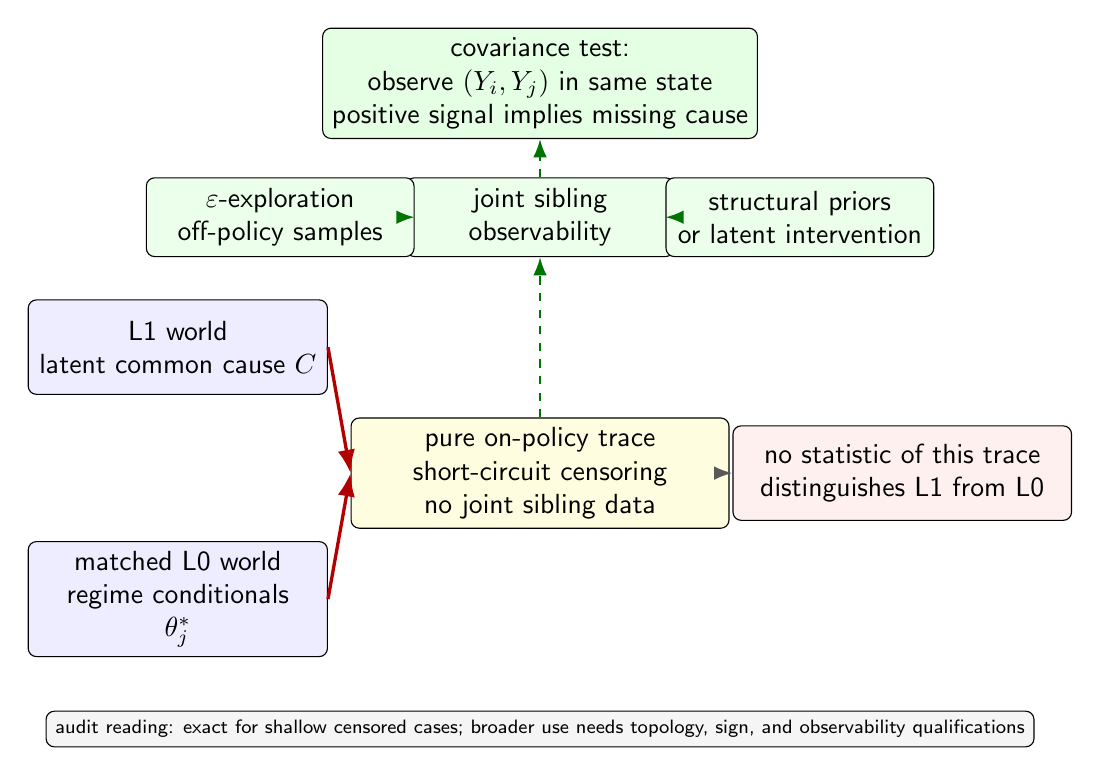
\begin{tikzpicture}[
  font=\sffamily,
  world/.style={draw, rounded corners=3pt, align=center, minimum width=38mm, minimum height=12mm, fill=white},
  trace/.style={draw, rounded corners=3pt, align=center, minimum width=48mm, minimum height=14mm, fill=yellow!12},
  route/.style={draw, rounded corners=3pt, align=center, minimum width=34mm, minimum height=10mm, fill=green!8},
  note/.style={align=center, font=\sffamily\scriptsize},
  arrow/.style={-Latex, thick, draw=black!65},
  same/.style={-Latex, very thick, draw=red!70!black},
  escape/.style={-Latex, thick, dashed, draw=green!45!black}
]

\node[world, fill=blue!7] (l1) at (0,1.6)
  {L1 world\\latent common cause $C$};
\node[world, fill=blue!7] (l0) at (0,-1.6)
  {matched L0 world\\regime conditionals\\$\theta_j^\ast$};

\node[trace] (policy) at (4.6,0)
  {pure on-policy trace\\short-circuit censoring\\no joint sibling data};
\node[world, fill=red!6, minimum width=43mm] (nog) at (9.2,0)
  {no statistic of this trace\\distinguishes L1 from L0};

\draw[same] (l1.east) -- (policy.west);
\draw[same] (l0.east) -- (policy.west);
\draw[arrow] (policy) -- (nog);

\node[route] (joint) at (4.6,3.25)
  {joint sibling\\observability};
\node[route] (prior) at (7.9,3.25)
  {structural priors\\or latent intervention};
\node[route] (explore) at (1.3,3.25)
  {$\varepsilon$-exploration\\off-policy samples};

\draw[escape] (policy.north) -- (joint.south);
\draw[escape] (joint.east) -- (prior.west);
\draw[escape] (joint.west) -- (explore.east);

\node[trace, fill=green!10, minimum width=50mm] (cov) at (4.6,4.95)
  {covariance test:\\observe $(Y_i,Y_j)$ in same state\\positive signal implies missing cause};
\draw[escape] (joint) -- (cov);

\node[note, fill=gray!8, draw, rounded corners=3pt, minimum width=95mm] at (4.6,-3.25)
  {audit reading: exact for shallow censored cases; broader use needs topology, sign, and observability qualifications};

\end{tikzpicture}
\end{document}
